
\documentclass[fleqn,addpoints]{exam}

\usepackage{units} 
\usepackage{graphicx}
\usepackage[fleqn]{amsmath}
\usepackage{cancel}
\usepackage{float}
\usepackage{mdwlist}
\usepackage{booktabs}
\usepackage{polynom}
\usepackage{caption}
\usepackage{fullpage}
\usepackage{comment}
\usepackage{enumerate}
\usepackage{parskip}
\usepackage{xfrac}

\newcommand{\degree}{\ensuremath{^\circ}} 
\everymath{\displaystyle}

% \printanswers
\excludecomment{comment}

\ifprintanswers 
  \usepackage{2in1, lscape} 
\fi

\author{}
\date{October 9, 2013}
\title{Math 142 \\ Chapter Five Exam}

\begin{document}

  \maketitle

  % \begin{center}
  %   \gradetable[h][pages]
  %   \bonusgradetable[h][pages]
  % \end{center}

  \section{Questions}

  \begin{questions}
    
    \question[6]
      If $\left( \frac{2}{3}, - \frac{\sqrt{5}}{3} \right)$ is the terminal point determined by $t$, find the values of
      all six trigonometric functions. 
      
      \begin{solution}
        \begin{tabular}[H]{cccccc}
          \toprule
          $\sin t$               & $\cos t$      & $\tan t$               & $\csc t$                 & $\sec t$      & $\cot t$ \\
          \midrule
          $- \frac{\sqrt{5}}{3}$ & $\frac{2}{3}$ & $- \frac{\sqrt{5}}{2}$ & $- \frac{3 \sqrt{5}}{5}$ & $\frac{2}{3}$ & $- \frac{\sqrt{5}}{3}$ \\
          \bottomrule
        \end{tabular}
      \end{solution}

    \question[8]
      If $\cot t = - \frac{1}{3}$ and $t$ is in quadrant IV, find the values of $\sin t$, $\cos t$, $\tan t$.

      \begin{solution}
        First find the terminal point.  Since the point is in quadrant IV, the $y$ coordinate is negative and the $x$
        coordinate is positive.

        \begin{align*}
          \frac{x}{y}  & = \frac{1}{3} \\
          y            & = 3x \\
          \\
          x^2 + y^2    & = 1 \\
          x^2 + (3x)^2 & = 1 \\
          10 x^2       & = 1 \\
          x            & = \frac{\sqrt{10}}{10} \\
          \\
          y            & = -3x \\
                       & = -\frac{3 \sqrt{10}}{10}  \\
        \end{align*}

        The terminal point is: $\left( \frac{\sqrt{10}}{10}, -\frac{3 \sqrt{10}}{10} \right)$.

        The values of the functions are:

        \begin{center}
          \begin{tabular}[H]{cccccc}
            \toprule
            $\sin t$                  & $\cos t$               & $\tan t$ \\
            \midrule
            $-3 \frac{\sqrt{10}}{10}$ & $\frac{\sqrt{10}}{10}$ & $-3$     \\
            \bottomrule
          \end{tabular}
        \end{center}

      \end{solution}

    \question Find the exact value of each expression.
      \begin{parts}

        \part[2] $\sin \frac{7 \pi}{6}$
          \begin{solution}
            $\sin \frac{7 \pi}{6} = - \frac{1}{2}$
          \end{solution}

        \part[2] $\cot \frac{3 \pi}{4}$
          \begin{solution}
            $\cot \frac{3 \pi}{4} = -1$
          \end{solution}

        \part[2] $\csc \frac{5 \pi}{3}$
          \begin{solution}
            $\csc \frac{5 \pi}{3} = - \frac{ 2 \sqrt{3}}{3}$
          \end{solution}

        \part[2] $\cos \frac{17 \pi}{2}$
          \begin{solution}
            $\cos \frac{17 \pi}{2} = \cos \left( \frac{\pi}{2} + 8 \pi \right) = \cos \frac{\pi}{2} = 0$
          \end{solution}

      \end{parts}

    \question
      \begin{parts}
        \part[5] Express $\csc x$ in terms of $\cos x$ if the  terminal point is in quadrant II.
          \begin{solution}
            \begin{align*}
              \csc^2 x  & = \frac{1}{\sin^2 x} \\
                        & = \frac{1}{1 - \cos^2 x} \\
              \csc x    & = \pm \frac{1}{ \sqrt{1 - \cos^2 x} } \\
            \end{align*}

            Cosecant is positive in quadrant II, so in quadrant II:
            \[
              \csc x = \frac{1}{ \sqrt{1 - \cos^2 x} } 
            \]
          \end{solution}

        \part[8] Express $\tan x$ in terms of $\csc x$ if the terminal point is in quadrant IV.
          \begin{solution}
            \begin{align*}
              \tan^2 x & = \frac{\sin^2 x}{\cos^2 x} \\
                       & = \frac{\sin x}{1 - \sin^2 x} \\
                       & = \frac{1}{\csc^2 x (1 - \sin^2 x)} \\
                       & = \frac{1}{\csc^2 x - 1} \\
              \tan x   & = \frac{1}{\sqrt{\csc^2 x - 1}} \\
            \end{align*}

            Tangent is negative in quadrant IV, so in quadrant IV:
            \[
              \tan x = - \frac{1}{\sqrt{\csc^2 x - 1}}
            \]
          \end{solution}

      \end{parts}
    
    \question $f(x) = - 10 \sin \left( 3x - \frac{\pi}{5} \right)$
      \begin{parts}
        \part[2] What is the amplitude?
        \part[2] What is the period?
        \part[3] What is the phase shift?
      \end{parts}

    \pagebreak

    \question[10]
      Find an equation for this graph.
      
      \begin{figure}[H]
        \centering
        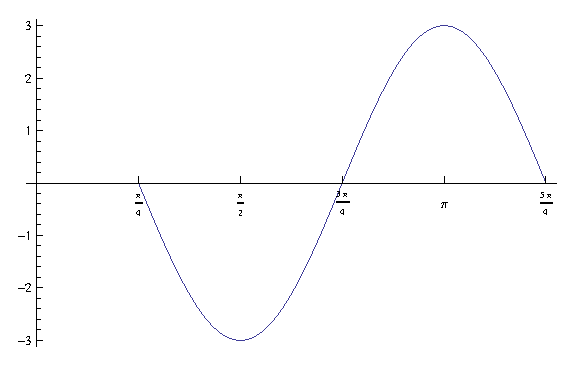
\includegraphics[scale=0.7]{find_equation.eps}
        \caption{Find the equation}
      \end{figure}

      \begin{solution}
        \begin{itemize*}
          \item The period is $\pi$
          \item The amplitude is 3
          \item The shape is an inverted sine graph
        \end{itemize*}

        The equation is:
        \[
          f(x) = - 3 \sin 2 \left( x - \frac{\pi}{4} \right) \\
        \]

      \end{solution}

    \question[10]
      Find the period and graph:
      \[
        f(x) = 5 \sin \left( \frac{1}{2} x - \frac{\pi}{3} \right)
      \]

      \begin{solution}
        \[
          f(x) = 5 \sin \left[ \frac{1}{2} \left( x - \frac{2 \pi}{3} \right) \right]
        \]

        \begin{figure}[H]
          \centering
          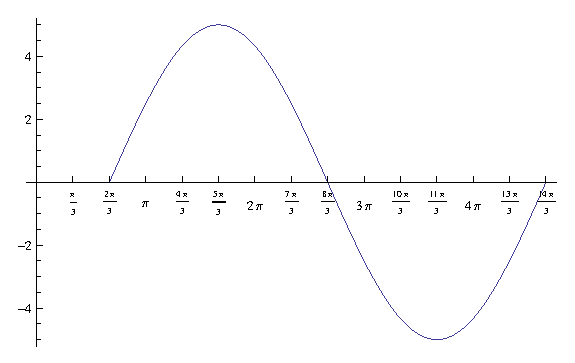
\includegraphics{graph1.eps}
          \caption{$f(x) = 5 \sin \left( \frac{1}{2} x - \frac{\pi}{3} \right)$}
        \end{figure}

      \end{solution}

    \question[10]
      Find the period and graph:
      \[
        f(x) = \cot \left( \pi x + \frac{\pi}{4} \right)
      \]

      \begin{solution}
        \[
          f(x) = \cot \left( \pi x + \frac{\pi}{4} \right) = \cot \left[ \pi \left( x + \frac{1}{4} \right) \right ]
        \]

        \begin{figure}[H]
          \centering
          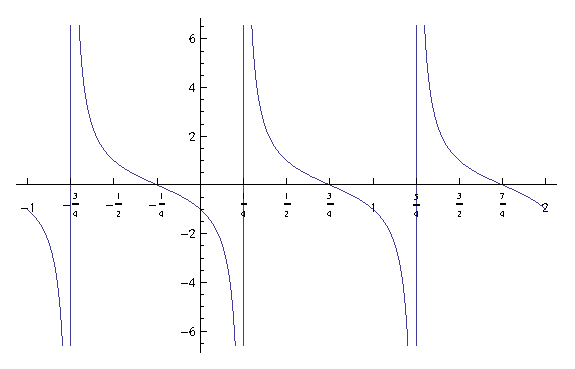
\includegraphics{graph2.eps}
          \caption{$f(x) = \cot \left( \pi x + \frac{\pi}{4} \right)$}
        \end{figure}

      \end{solution}

    \question[10]
    Find the period and graph:
      \[
        f(x) = - \sec 2x
      \]

      \begin{solution}
        \begin{figure}[H]
          \centering
          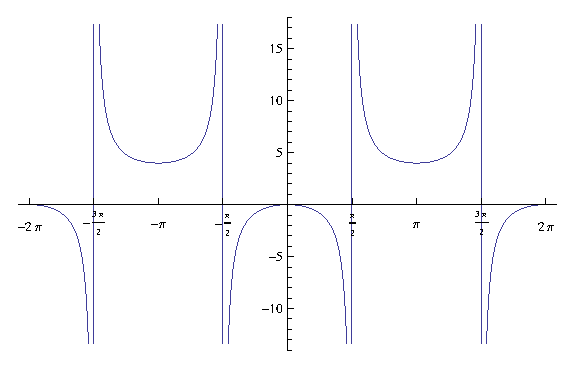
\includegraphics[scale=1.0]{graph3.eps}
          \caption{$f(x) = - \sec 2x $}
        \end{figure}

      \end{solution}

    \question[8]
      A mass is suspended on a spring.  The mass is raised to 10 cm above its rest position and released at time $t =
      0$.  One second after the mass is released it reaches its lowest point.  Find an equation for the motion of the mass.
      
      \begin{solution}
        \begin{itemize*}
          \item Since the mass was initially 10 cm above the rest position, the amplitude is 10.
          \item The motion is starting out at the maximum amplitude at time zero, so the motion follows a cosine
            function.
          \item Since half a cycle takes 1 second, a full cycle takes 2 seconds and $\omega = \frac{2 \pi}{2} = \pi$ 
        \end{itemize*}

        The equation is:
        \[
          h(t) = 10 \cos \pi t
        \]

        \begin{figure}[H]
          \centering
          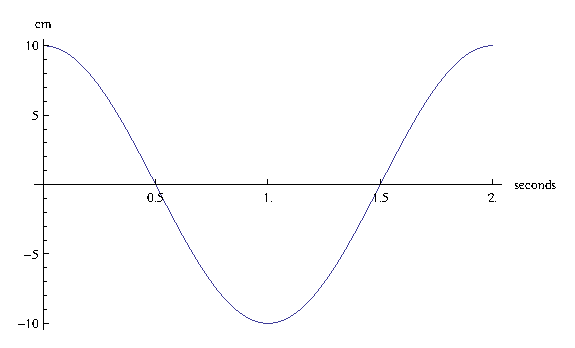
\includegraphics[scale=1.0]{spring.eps}
          \caption{Weight Height}
        \end{figure}

      \end{solution}

    \question[10] 
      Harry and Ron are hovering 1 foot off the ground in the Flying Ford Anglia before setting off for Hogwarts.  The
      wheels have a radius of 9 inches and are spinning at a steady 3 revolutions per second.  Find an equation for the
      height in inches from the ground of a Cornish Pixie squashed on the bottom of one of the wheels.

      \begin{solution}
        \begin{itemize*}
          \item The angular velocity is: $\omega = 3 \cdot 2 \pi = 6 \pi$
          \item The offset is the height off the ground plus the radius or 21 inches.
          \item The amplitude is $\unit[9]{inches}$
        \end{itemize*}

        The equation is: $h(t) = 21 + 9 \sin 6 \pi t$ 

        \begin{figure}[H]
          \centering
          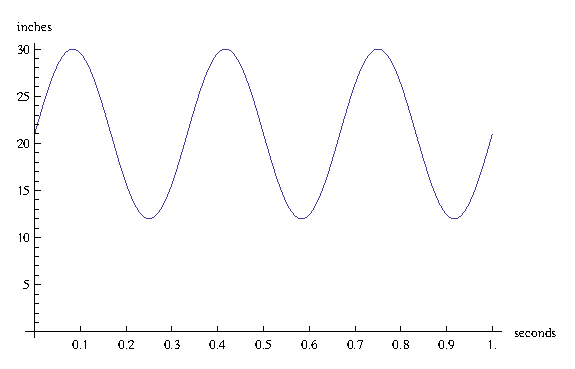
\includegraphics[scale=1.0]{graph5.eps}
          \caption{Cornish Pixie Height}
        \end{figure}

      \end{solution}

    \uplevel{ \section{Extra Credit} }

    \bonusquestion
      An astronaut takes a pendulum clock from earth to the planet Zircon where he finds that it runs more slowly
      because of the low Zirconian gravity.      He coordinates with mission control and finds that his clock is running
      15 minutes slow each hour.  In other words, after the clock on earth says one hour has elapsed, the clock on
      Zircon says only 45 minutes have elapsed.

      On earth, the equation for the pendulum's motion is:
      \[
        h(t) = \cos 2 \pi t
      \]

      \begin{parts}
          
        \bonuspart[8]
          What is the equation for the motion on Zircon?

          \begin{solution}
            On earth, the period is:
            \[
              p_e = \frac{2 \pi}{2 \pi} = \unit[1]{s}
            \]

            45 Zircon periods are equal to 60 earth periods:
            \begin{align*}
              45 p_z & = 60 p_e \\
              p_z    & = \frac{ 60 p_e }{45} \\
                     & = \frac{ 4 p_e }{3} \\
            \end{align*}

            Find $\omega_z$:
            \begin{align*}
              \omega_z & = \frac{2 \pi}{p_z} \\
                       & = 2 \pi \cdot \frac{3}{4} \\
                       & = \frac{3 \pi}{2} \\
            \end{align*}

            The Zircon equation for the motion is:
            \[
              h_z = 5 \cos \frac{3 \pi}{2} t
            \]

          \end{solution}

        \bonuspart[4]
          For a pendulum, $\omega = \sqrt{ \sfrac{g}{L}}$ where $g$ is the acceleration due to gravity and
          $L$ is the length of the pendulum.

          On earth: $g_e \approx \unit[10]{m/s^2}$.  What is the value of $g$ on Zircon?

          \begin{solution}
            Find the length of the pendulum:
            \begin{align*}
              \sqrt{ \frac{10}{L} } & = 2 \pi \\
              \frac{10}{L}          & = 4 \pi^2 \\
              L                     & = \frac{5}{2 \pi^2} \\
            \end{align*}

            Find $g_z$:
            \begin{align*}
              \frac{3 \pi}{2} & = \sqrt{ \frac{2 \pi^2 g_z}{5}} \\
              \frac{3}{2}     & = \sqrt{ \frac{2 g_z}{5}} \\
              \frac{9}{4}     & = \frac{2 g_z}{5} \\
              g_z             & = \frac{45}{8} \\
            \end{align*}

          \end{solution}
      \end{parts}

  \end{questions}
\end{document}

